\section{Mikroservisų sistemos vidinių integracijų tipai}
Pagal Sam Newman knygą „Building Mircroservices: Designing Fine-Grained Systems“ \cite{Bk2} vienas iš pagrindinių
integracijų projektavimo apsektų yra stengtis išvengti nesuderinamų pakeitimų (angl. \textit{„breaking changes“}).
Norint išvengti tokių pakeitimų, reikia rinktis tokį technologinį sprendimą, kad pakeitus vieno mikroserviso grąžinamų
duomenų struktūrą, kiti servisai be pakeitimų veiktų ir galėtų gauti duomenis.
Sam Newman teigimu „tinkamos integracijos pasirinkimas yra pats svarbiausias technologinis su mikroservisais susijęs dalykas“.
Todėl labai svarbu yra pasirinkti tinkamą integracijų tipą, nes nuo to priklauso kiek daug problemų sukels naujų funkcionalumų kūrimas.
Autorius išskyria keletą skirtingų mikroservisų komunikavimo tipų, kuriuos ir aptarsime:
\begin{enumerate}
	\item Servisų jungimas per duomenų bazę.
	\item Sinchroninės užklausos/atsakymo (angl. \textit{„request/response“}) integracijos.
	\item Asinchroninės įvykiais paremtos (angl. \textit{„event-based“}) integracijos.
\end{enumerate}

\break

\subsection{Servisų komunikavimas per duomenų bazę}
Šis integracinis tipas yra paremtas vienos bendros duomenų bazės naudojimu per keletą skirtingų mikroservisų.
Šis tipas ypatingas tuo, kad kiekvienas mikroservisas turi priėjimą prie tų pačių resursų, tik modifikuoja resursus
už juos atsakingi mikroservisai. Mikroservisų sistemos komunikavimo per duomenų bazę schema (\ref{img:db-communication} pav.):

\begin{figure}[H]
  \centering
  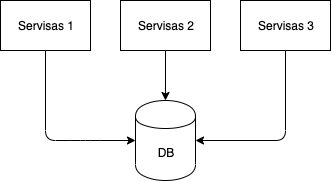
\includegraphics[scale=0.8]{img/db-communication}
  \caption{Mikroservisų komunikavimas duomenų bazės pagalba.}
  \label{img:db-communication}
\end{figure}

Svarbu paminėti, jog toks komunikacijų tipas yra labai nesaugus ir duomenų migravimas kuriant stambesnius funkcionalumus yra neišvengiamas.
Pačio Sam Newman, knygos \cite{Bk2} autoriaus, nuomone, tai yra praščiausias komunikavimo būdas ir stipriai nerekomenduojamas.
Dėl šios priežasties komunikavimo per bendrą duomenų bazę daugiau šiame darbe nenagrinėsime.